\documentclass[12pt,a4paper]{article}
\usepackage[T1]{fontenc}
\usepackage{graphicx}
\usepackage{float}
\usepackage{amsmath}
\usepackage{amssymb}
\usepackage{geometry}
\usepackage{hyperref}
\usepackage{listings}
\usepackage{xcolor}
\usepackage[utf8]{inputenc}
\usepackage[polish]{babel}
\lstset{
  language=Python,
  basicstyle=\ttfamily\small,
  keywordstyle=\color{blue}\bfseries,
  commentstyle=\color{gray}\itshape,
  stringstyle=\color{orange},
  showstringspaces=false,
  showspaces=false,
  keepspaces=true,
  columns=fixed,
  breaklines=true,
  breakatwhitespace=true,
  breakindent=10pt,
  postbreak=\mbox{\textcolor{gray}{\(\hookrightarrow\)\space}}
}

\geometry{margin=1in}

\title{Explicable Low-Code/No-Code System\\Wspierany przez Model Językowy}
\author{Maciej Trzaskacz}
\date{\today}

\begin{document}

\maketitle

\begin{abstract}
Niniejszy raport prezentuje system Explainable Low-Code/No-Code (LC/NC) wspierany przez model językowy, którego celem jest nie tylko generowanie prototypów aplikacji na podstawie promptu użytkownika, ale także wyjaśnianie, które fragmenty promptu wpłynęły na konkretne cechy aplikacji. System dekomponuje prompt na fragmenty, generuje strukturę aplikacji oraz oblicza atrybucję wpływu fragmentów metodą inspirowaną SHAP. Raport zawiera opis czterech pytań badawczych, wykonanych eksperymentów oraz wstępne wyniki.
\end{abstract}

\section{Wprowadzenie}

Generowanie aplikacji przy użyciu technologii Low-Code/No-Code (LC/NC) staje się coraz bardziej popularne. Jednak użytkownicy często nie rozumieją, jak ich intencje wyrażone w promptach zostają przetłumaczone na konkretne cechy aplikacji. Brak przejrzystości w tym procesie utrudnia diagnozowanie problemów, iteracyjne ulepszanie promptów oraz budowanie zaufania do systemu.

Niniejszy projekt ma na celu opracowanie systemu, który łączy explicability z generowaniem LC/NC aplikacji. System wykorzystuje:
\begin{itemize}
    \item Dekomponowanie promptu na mniejsze, dyskretne fragmenty
    \item Generowanie struktury aplikacji (encje, operacje, storage)
    \item Obliczanie atrybucji wpływu fragmentów promptu na konkretne cechy aplikacji
    \item Wizualizację wyjaśnień w formie grafów zależności i raportów tekstowych
\end{itemize}

\section{Pytania Badawcze}

Projekt opiera się na czterech głównych pytaniach badawczych:

\begin{description}
    \item[RQ1:] Czy atrybucja fragmentów promptu do cech aplikacji (prompt-to-feature attribution) poprawia zrozumienie i kontrolę nad generowanymi prototypami LC/NC?
    
    \item[RQ2:] Na ile dokładnie metoda atrybucji (SHAP-inspired) identyfikuje fragmenty promptu odpowiedzialne za konkretne feature'y aplikacji?
    
    \item[RQ3:] Czy wyjaśnienia oparte na atrybucji pomagają użytkownikom skuteczniej diagnozować i poprawiać prompty (prompt refinement)?
    
    \item[RQ4:] Jaki jest kompromis między kosztem obliczeniowym a jakością wyjaśnień w proponowanym podejściu?
\end{description}


\section{Metodologia}

\subsection{Ogólne Podejście}

System działa w następujących krokach:

\begin{enumerate}
    \item \textbf{Dekomponowanie promptu} --- użytkownika prompt dzielony jest na dyskretne fragmenty, każdy odpowiadający jednemu wymaganiu
    \item \textbf{Generowanie architektury} --- na podstawie pełnego promptu generowana jest struktura aplikacji (encje, relacje, operacje)
    \item \textbf{Obliczanie atrybucji} --- dla każdego fragmentu obliczany jest jego wpływ na każdą cechę aplikacji
    \item \textbf{Wizualizacja wyników} --- wyniki prezentowane są użytkownikowi w formie wizualnej i tekstowej
\end{enumerate}

\subsection{Metoda Atrybucji}

Projekt wykorzystuje metodę inspirowaną SHAP (SHapley Additive exPlanations), zmodyfikowaną dla kontekstu LC/NC:

\begin{equation}
\phi_i(\text{feature}) = \frac{1}{m} \sum_{S \subset F \setminus \{i\}} \left[ v(S \cup \{i\}) - v(S) \right]
\end{equation}

gdzie:
\begin{itemize}
    \item $\phi_i$ --- atrybucja fragmentu $i$
    \item $F$ --- zbiór wszystkich fragmentów
    \item $v(S)$ --- wartość cechy dla podzbioru fragmentów $S$
\end{itemize}

\section{Feature'y Systemu}
Na podstawie architektury generowanej przez model językowy, definiujemy zestaw cech (feature'ów) aplikacji, które będą analizowane pod kątem atrybucji:

\subsection{Feature'y Funkcjonalne}
\begin{itemize}
    \item \texttt{has\_offline\_storage} --- aplikacja pracuje bez internetu / tryb offline
    \item \texttt{has\_reminders} --- użytkownik otrzymuje przypomnienia (czasowe)
    \item \texttt{has\_notifications} --- powiadomienia push/systemowe
    \item \texttt{has\_authentication} --- logowanie / konta użytkowników
    \item \texttt{has\_sharing} --- możliwość dzielenia się danymi
    \item \texttt{has\_search} --- możliwość wyszukiwania danych
\end{itemize}

\subsection{Feature'y Strukturalne}
\begin{itemize}
    \item \texttt{num\_entities} --- liczba encji w modelu danych
    \item \texttt{num\_relationships} --- liczba relacji między encjami
    \item \texttt{has\_user\_entity} --- obecność encji User
    \item \texttt{has\_task\_entity} --- obecność encji Task
\end{itemize}

\subsection{Feature'y Operacyjne}
\begin{itemize}
    \item \texttt{has\_create, has\_read, has\_update, has\_delete} --- operacje CRUD
    \item \texttt{has\_notify\_operation} --- operacja powiadomienia
\end{itemize}

\subsection{Feature'y Architektoniczne}
\begin{itemize}
    \item \texttt{uses\_local\_storage} --- magazynowanie danych lokalnie
    \item \texttt{uses\_database} --- trwałe przechowywanie strukturyzowane
    \item \texttt{uses\_api} --- komunikacja z zewnętrznym/backend API
\end{itemize}

\section{Implementacja}
System zaimplementowano w Pythonie. Do testów użyto lokalnego API Ollama (model Mistral), a dane architektury są wymieniane w formacie JSON. Metodologia atrybucji opiera się na podejściu inspirowanym SHAP (sampling subsets / leave-one-out). Kod źródłowy dostępny pod adresem \url{https://github.com/matrzask/LCNC}.

\subsection{Stack i pliki}
\begin{itemize}
    \item \textbf{Python 3.12}
    \item Zestaw modułów: \texttt{requests}, \texttt{tqdm} (opcjonalnie), \texttt{networkx}, \texttt{matplotlib}, \texttt{pandas}, \texttt{numpy}
    \item Główne pliki w repozytorium: \texttt{lcnc.py}, \texttt{visualize.py}
\end{itemize}

\subsection{Fragmenty kodu}
Poniżej znajdują się skrócone i istotne fragmenty implementacji wykorzystane w projekcie (pełna implementacja jest w \texttt{lcnc.py} i \texttt{visualize.py}).

\subsubsection{Dekompozycja promptu i generowanie architektury}
\begin{lstlisting}[language=Python]
def extract_prompt_fragments(user_prompt: str) -> list:
    """
    Dzieli zlozony prompt uzytkownika na mniejsze fragmenty,
    z ktorych kazdy odpowiada jednej funkcjonalnosci lub wymaganiu.
    """
    decomposition_prompt = f"""
    You are a system that extracts requirement fragments from a user prompt.

    STRICT RULES (CRITICAL):
    - DO NOT paraphrase.
    - DO NOT summarize.
    - DO NOT translate.
    - DO NOT reorder words inside fragments.
    - DO NOT merge multiple requirements into one.
    - Each fragment must correspond to ONE distinct requirement or feature.
    - Keep fragments as close as possible to the original wording.
    - If a sentence contains multiple requirements, split it into smaller parts.

    OUTPUT FORMAT:
    - Return ONLY fragments
    - One fragment per line
    - NO bullets
    - NO numbering
    - NO explanations

    USER PROMPT:
    \"\"\"{user_prompt}\"\"\"
    """
    
    raw_output = call_ollama(decomposition_prompt, temperature=0.0)
    
    # czyszczenie
    fragments = []
    for line in raw_output.split("\n"):
        line = line.strip()
        if line:
            fragments.append(line)
            
    return fragments

def generate_architecture(user_prompt: str) -> dict:
    """
    Generuje strukture architektury low-code/no-code
    na podstawie promptu uzytkownika,
    zgodnie z scisle okreslonymi regulami i formatem JSON.
    """
    architecture_prompt = """
    You are a system that generates a STRUCTURED low-code/no-code application architecture from a user prompt.

    Your output will be used for automated analysis, so it must be STRICT, COMPLETE, and MACHINE-READABLE.

    ========================================
    CRITICAL RULES (DO NOT VIOLATE)
    ========================================
    - Output MUST be valid JSON.
    - DO NOT include explanations.
    - DO NOT include comments.
    - DO NOT include any text outside JSON.
    - DO NOT infer features not explicitly supported by the prompt.
    - DO NOT add "best practices" or optional features.
    - ONLY include elements that are clearly implied by the prompt.
    - If something is not mentioned, DO NOT include it.

    ========================================
    OUTPUT FORMAT (STRICT JSON)
    ========================================

    {{
    "entities": [
        {{
        "name": "EntityName",
        "attributes": ["attribute1", "attribute2"]
        }}
    ],
    "relationships": [
        {{
        "from": "EntityA",
        "to": "EntityB",
        "type": "relationship_type"
        }}
    ],
    "operations": [
        {{
        "type": "operation_type",
        "entity": "EntityName"
        }}
    ],
    "features": {{
        "has_offline_storage": 0,
        "has_reminders": 0,
        "has_notifications": 0,
        "has_authentication": 0,
        "has_sharing": 0,
        "has_search": 0
    }},
    "architecture": {{
        "uses_local_storage": 0,
        "uses_database": 0,
        "uses_api": 0
    }}
    }}

    ========================================
    FEATURE DEFINITIONS (IMPORTANT)
    ========================================
    Set values to 1 ONLY if clearly supported by the prompt.

    - has_offline_storage -> app works without internet / offline mode
    - has_reminders -> user gets reminders (time-based)
    - has_notifications -> push/system notifications
    - has_authentication -> login/user accounts
    - has_sharing -> sharing data with others
    - has_search -> ability to search data

    ARCHITECTURE:
    - uses_local_storage -> data stored locally on device
    - uses_database -> persistent structured storage
    - uses_api -> external or backend API communication

    ========================================
    OPERATION RULES
    ========================================
    Include operations ONLY if implied.
    Operation types should be standardized as:
    - create
    - read
    - update
    - delete
    - notify (only if reminders/notifications exist)
    Also include the associated entity for each operation.

    ========================================
    ENTITY RULES
    ========================================
    - Only include entities clearly present in the prompt.
    - Use simple names (User, Task, Note, etc.)
    - Do not invent entities.

    ========================================
    USER PROMPT
    ========================================
    \"\"\"{user_prompt}\"\"\"
    """.format(user_prompt=user_prompt)

    raw_output = call_ollama(architecture_prompt, temperature=0.0, response_format="json")

    try:
        return json.loads(raw_output)
    except json.JSONDecodeError:
        try:
            return parse_first_json(raw_output)
        except Exception:
            return None
\end{lstlisting}

\subsubsection{Ekstrakcja wektora cech}
\begin{lstlisting}[language=Python]
def extract_feature_vector(arch: dict) -> dict:
    """
    Zamienia architekture JSON na plaski feature vector.
    """

    features = arch.get("features", {})
    architecture = arch.get("architecture", {})
    entities = arch.get("entities", [])
    relationships = arch.get("relationships", [])
    operations = arch.get("operations", [])

    feature_vector = {
        # === funkcjonalne ===
        "has_offline_storage": int(features.get("has_offline_storage", 0)),
        "has_reminders": int(features.get("has_reminders", 0)),
        "has_notifications": int(features.get("has_notifications", 0)),
        "has_authentication": int(features.get("has_authentication", 0)),
        "has_sharing": int(features.get("has_sharing", 0)),
        "has_search": int(features.get("has_search", 0)),

        # === strukturalne ===
        "num_entities": len(entities),
        "num_relationships": len(relationships),
        "has_user_entity": int(any(e["name"].lower() == "user" for e in entities)),
        "has_task_entity": int(any(e["name"].lower() == "task" for e in entities)),

        # === operacyjne ===
        "has_create": int(any(op["type"] == "create" for op in operations)),
        "has_read": int(any(op["type"] == "read" for op in operations)),
        "has_update": int(any(op["type"] == "update" for op in operations)),
        "has_delete": int(any(op["type"] == "delete" for op in operations)),
        "has_notify_operation": int(any(op["type"] == "notify" for op in operations)),

        # === architektoniczne ===
        "uses_local_storage": int(architecture.get("uses_local_storage", 0)),
        "uses_database": int(architecture.get("uses_database", 0)),
        "uses_api": int(architecture.get("uses_api", 0)),
    }

    return feature_vector
\end{lstlisting}

\subsubsection{SHAP-inspired: sampling subsets}
\begin{lstlisting}[language=Python]
def shap_sampling_attribution(fragments, generate_arch_fn, samples=10):
    """
    SHAP-like attribution: leave-one-out
    """

    # baseline
    full_arch = generate_arch_fn(prompt)
    full_features = extract_feature_vector(full_arch)

    attributions = {}

    for frag in fragments:
        reduced_fragments = [f for f in fragments if f != frag]
        reduced_prompt = " ".join(reduced_fragments)

        reduced_arch = generate_arch_fn(reduced_prompt)
        reduced_features = extract_feature_vector(reduced_arch)

        diff = feature_diff(full_features, reduced_features)

        attributions[frag] = diff

    return attributions
\end{lstlisting}

\subsection{Przykładowe wizualizacje}
Poniżej znajdują się przykładowe wykresy wygenerowane przez \texttt{visualize.py}.

\begin{figure}[H]
    \centering
    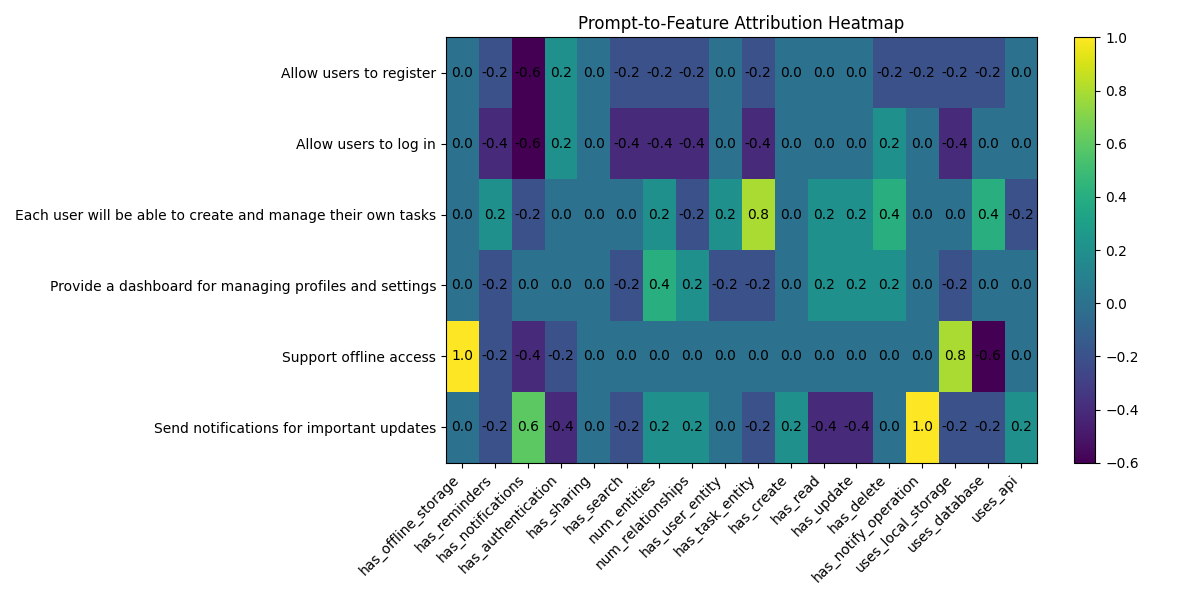
\includegraphics[width=0.8\textwidth]{plots/attribution_heatmap.png}
    \caption{Mapa atrybucji fragmentów do cech (heatmap).}
\end{figure}

\begin{figure}[H]
    \centering
    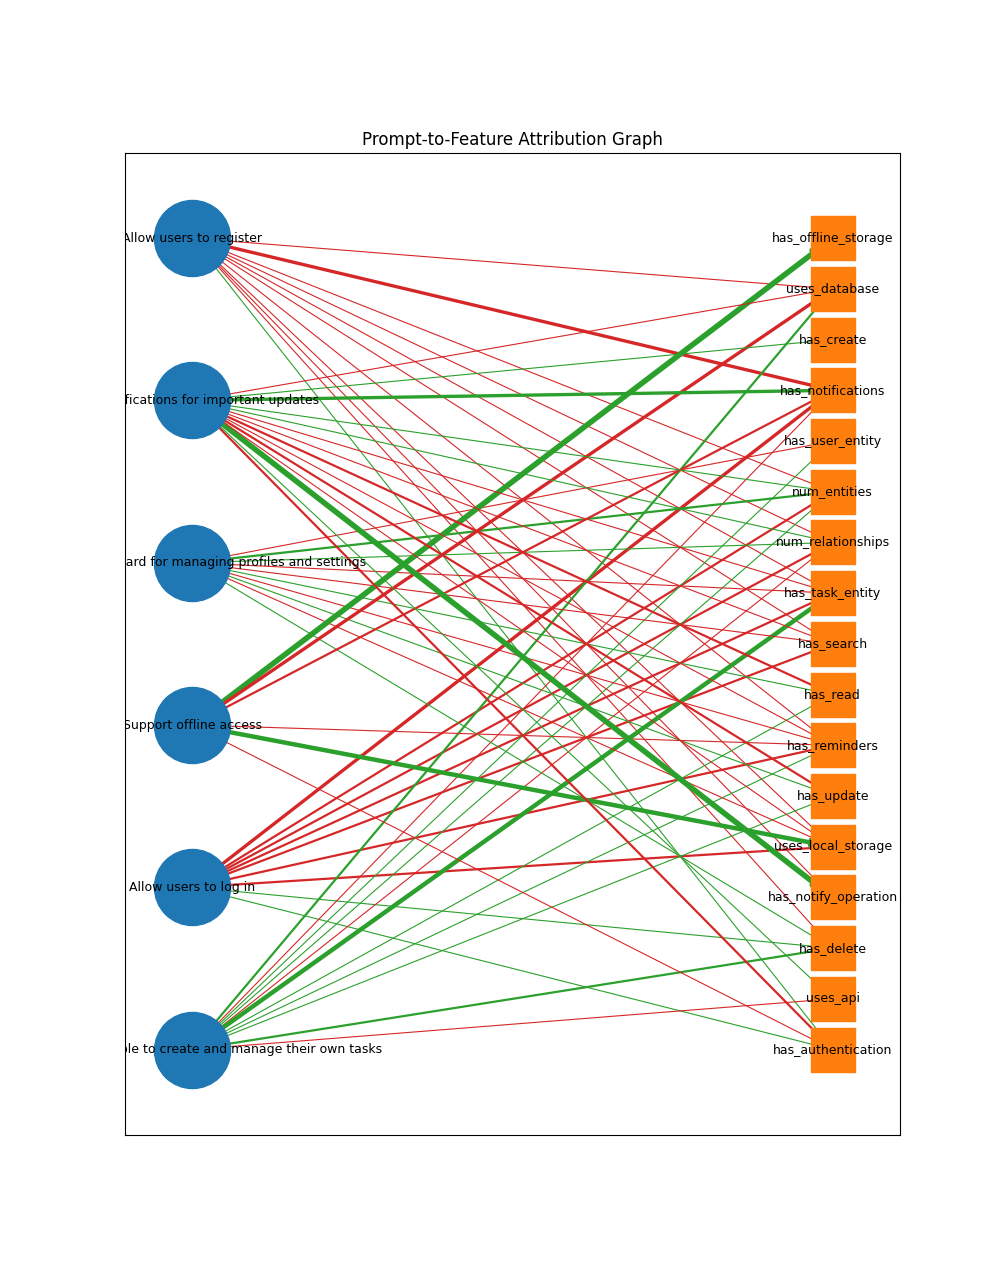
\includegraphics[width=0.8\textwidth]{plots/attribution_graph.png}
    \caption{Graf zależności fragmentów i cech (edge weight = siła wpływu).}
\end{figure}

\begin{figure}[H]
    \centering
    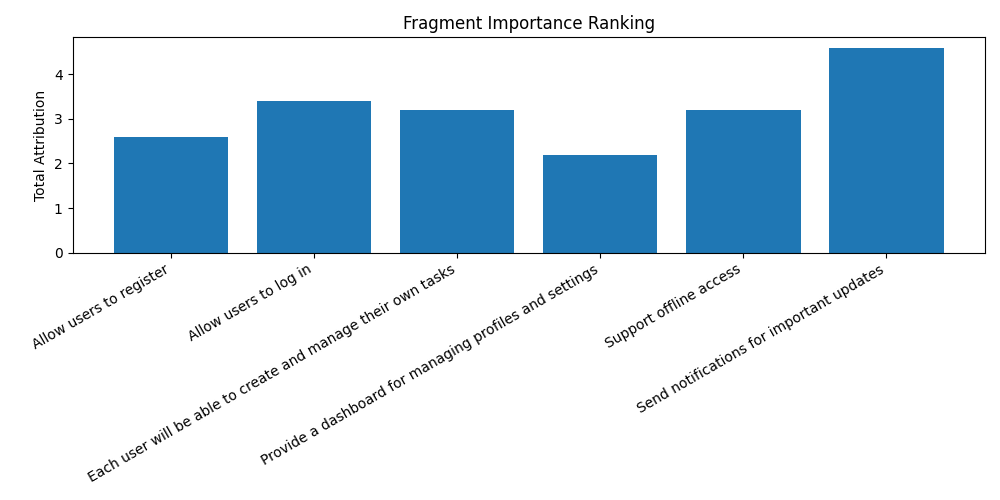
\includegraphics[width=0.8\textwidth]{plots/fragment_importance.png}
    \caption{Wykres słupkowy pokazujący sumaryczny wpływ każdego fragmentu na wszystkie cechy.}
\end{figure}

% \begin{figure}[H]
%     \centering
%     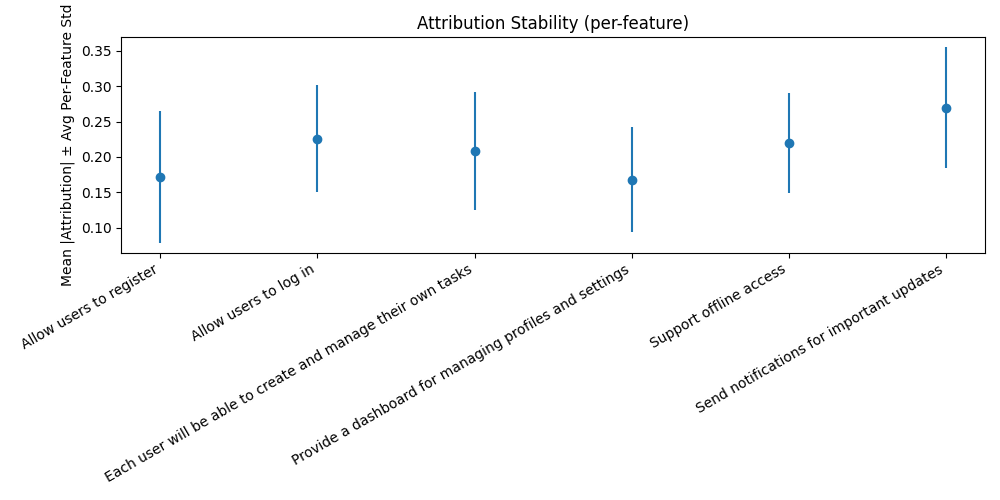
\includegraphics[width=0.8\textwidth]{plots/stability.png}
%     \caption{Wykres pokazujący stabilność atrybucji w zależności od liczby próbek.}
% \end{figure}

\section{Eksperymenty}

\subsection{Eksperyment 1: Dokładność Atrybucji (Feature Drop Rate)}

\paragraph{Cel:} Sprawdzenie, czy atrybucja identyfikuje fragmenty rzeczywiście wpływające na cechy aplikacji.

\paragraph{Metodyka:}
\begin{enumerate}
    \item Generowane są atrybucje dla wszystkich fragmentów promptu
    \item Usuwany jest fragment o \textbf{najwyższym} wpływie na wybraną cechę
    \item Usuwany jest \textbf{losowy} fragment (baseline)
    \item Porównywana jest zmiana wartości cechy w obu przypadkach
\end{enumerate}

\paragraph{Metryka:}
\begin{equation}
\text{Feature Drop Rate} = \frac{\text{Zmiana cechy (top frag)}}{\text{Zmiana cechy (random frag)}}
\end{equation}

Wartości wyższe od 1 wskazują, że fragment o najwyższej atrybucji ma większy wpływ niż losowy.

\vspace{1cm}

\paragraph{Wyniki:}
Na potrzeby eksperymentu uruchomiono analizę dla przykładowego promptu

\paragraph{Ranking fragmentów (skrót)}
Lista fragmentów z najwyższymi łącznymi score (suma bezwzględnych atrybucji):
\begin{itemize}
    \item "Send notifications for important updates" — Score: 6.6
    \item "Offline access support" — Score: 5.0
    \item "Collaborate on shared projects and tasks" — Score: 4.2
    \item "Encrypt and securely store user data in the cloud database" — Score: 3.4
    \item "Seamless and automatic data synchronization across multiple devices" — Score: 3.2
    \item "Secure authentication for user registration and login" — Score: 2.2
    \item "Manage own tasks with priorities and deadlines" — Score: 2.2
\end{itemize}

\paragraph{Usunięcie top vs losowego fragmentu}
Wyniki porównania:
\begin{itemize}
    \item Top fragment: "Send notifications for important updates" — liczba utraconych cech: 3
    \item Losowy fragment: "Role-based access control for different user types" — liczba utraconych cech: 0
\end{itemize}

Ponieważ w przypadku fragmentu losowego liczba utraconych cech wyniosła 0, bezpośredni iloraz w metryce Feature Drop Rate jest nieoznaczony; praktyczna interpretacja wyników pokazuje jednak, że usunięcie fragmentu wskazanego przez atrybucję prowadzi do istotnej utraty funkcjonalności (3 cechy), podczas gdy usunięcie fragmentu losowego nie zmienia wykrytych cech.

\paragraph{Dodatkowy przykład}
Przeprowadzono drugą próbę, z krótszym promptem testowym. Skrót wyników:
\begin{itemize}
    \item Ranking fragmentów (skrót):
    \begin{itemize}
        \item "Offline Access Support" — Score: 3.6
        \item "Real-Time Notifications" — Score: 3.0
        \item "Task Management Capabilities" — Score: 2.8
        \item "Cloud Data Synchronization" — Score: 2.8
        \item "Dashboard for Profile and Settings Management" — Score: 2.0
        \item "Role-Based Access Control" — Score: 2.0
        \item "User Authentication" — Score: 1.8
    \end{itemize}
    \item Porównanie usunięcia fragmentu top vs losowego:
    \begin{itemize}
        \item Top fragment: "Offline Access Support" — liczba utraconych cech: 3
        \item Losowy fragment: "Real-Time Notifications" — liczba utraconych cech: 2
    \end{itemize}
\end{itemize}

W obu przykładach usunięcie fragmentu o najwyższym score prowadziło do utraty większej liczby feature'ów niż usunięcie fragmentu losowego (3 vs 0 i 3 vs 2), co wspiera hipotezę, że atrybucja identyfikuje istotne fragmenty. Jednakże wariancja między eksperymentami pokazuje, że wynik zależy od konkretnej treści promptu i wyboru fragmentu losowego.

\subsection{Eksperyment 2: Użyteczność dla Refinementu Promptu}

\paragraph{Cel:} Sprawdzenie, czy wyjaśnienia oparte na atrybucji pomagają użytkownikom bardziej efektywnie ulepszać prompty.

\paragraph{Implementacja Aplikacji Webowej:}

Aplikacja webowa (ex2\_web\_app.py) została zbudowana przy użyciu Flask oraz Plotly i umożliwia interaktywny refinement promptów. Główne funkcjonalności:

\begin{itemize}
    \item \textbf{Interfejs użytkownika:} formularz do wpisania promptu i ustawienia liczby próbek dla SHAP-inspired atrybucji
    \item \textbf{Backend:} asynchroniczne przetwarzanie z aktualizacją progresu w czasie rzeczywistym
    \item \textbf{Wizualizacje:} 
    \begin{itemize}
        \item Heatmapa atrybucji fragmentów do cech aplikacji
        \item Wykres słupkowy pokazujący wykryte cechy (features) i architekturę
        \item Rozkład fragmentów i wygenerowanej struktury danych
    \end{itemize}
    \item \textbf{Sesje:} zapisywanie historii promptów użytkownika w formacie JSON
\end{itemize}

\begin{figure}[H]
    \centering
    \includegraphics[width=1\linewidth]{ex2_webui.png}
    \caption{Fragment interfejsu webowej aplikacji do interaktywnego refinementu promptów z heat-mapą atrybucji.}
    \label{fig:ex2_webui}
\end{figure}

\paragraph{Metodyka:}

Przeprowadzono dwie pary prób (próba 1 i próba 2) w dwóch wariantach:
\begin{itemize}
    \item \textbf{Z atrybucjami (att):} użytkownik otrzymywał wizualizacje pokazujące, które fragmenty promptu wpływają na konkretne cechy
    \item \textbf{Bez atrybucji (noatt):} użytkownik widział tylko architekturę, bez informacji o wpływie fragmentów
\end{itemize}

\paragraph{Metryki:}
\begin{itemize}
    \item Liczba iteracji potrzebna do osiągnięcia celu
    \item Rodzaj zmian wprowadzonych w każdej iteracji
    \item Uwagi użytkownika
\end{itemize}

\paragraph{Wyniki:}

\subparagraph{Próba 1: Osiągnięcie Brakujących Cech.}

\subparagraph{Cel:} uzyskać cechy \texttt{has\_authentication}, \texttt{has\_reminders},\\ \texttt{has\_notifications} oraz \texttt{uses\_local\_storage}.

\begin{itemize}
    \item \textbf{Bez atrybucji (noatt\_1):} 7 iteracji
    \begin{itemize}
        \item Startowy prompt: ``Stwórz aplikację do zarządzania zadaniami''
        \item Próbki bez atrybucji wymagały więcej iteracji i bardziej eksperymentalnych zmian w sformułowaniu
        \item Uwaga: trudność w osiągnięciu \texttt{has\_reminders}, wymagało kilku prób.
    \end{itemize}
    
    \item \textbf{Z atrybucjami (att\_1):} 5 iteracji
    \begin{itemize}
        \item Startowy prompt: identyczny jak wyżej
        \item Uwaga: W pierwszej próbie fragment uzyskał atrybucję \texttt{uses\_local\_storage} o wartości 1. Dało to wrażenie że nie trzeba tego precyzować w dalszych etapach, co było błędne.
    \end{itemize}
\end{itemize}

\vspace{1cm}

\subparagraph{Próba 2: Usunięcie Cechy przy Zachowaniu Funkcjonalności}

\subparagraph{Cel:} usunąć cechę \texttt{has\_authentication}, zachowując pozostałe funkcjonalności.

\begin{itemize}
    \item \textbf{Bez atrybucji (noatt\_2):} 5 iteracji
    \begin{itemize}
        \item Startowy prompt: ``Stwórz aplikację do zarządzania zadaniami dla użytkowników. Każdy użytkownik ma prywatny pulpit z listą zadań, osobistymi ustawieniami i możliwością synchronizacji danych między urządzeniami. Aplikacja powinna umożliwiać tworzenie, edytowanie i przypominanie terminów oraz wysyłać powiadomienia o ważnych wydarzeniach. Użytkownicy mogą udostępniać wybrane zadania współpracownikom.''
        \item Uwaga w iteracji 2: aplikacja nie zawierała autoryzacji, ale też nie zawierała możliwości dzielenia się zadaniami.
        \item Bez atrybucji potrzeba wprowadzania bardziej drastycznych zmian, zmusza do eksperymentowania.
    \end{itemize}
    
    \item \textbf{Z atrybucjami (att\_2):} 3 iteracje
    \begin{itemize}
        \item Startowy prompt: identyczny jak wyżej
        \item Uwaga w iteracji 2: System niepoprawnie rozdzielił prompt na fragmenty; trzeba było powtórzyć iterację. Gdyby nie to, zadanie udałoby się po jednej próbie.
        \item Obserwacja: atrybucja pozwala skupić się na kluczowych fragmentach promptu.
    \end{itemize}
\end{itemize}

\paragraph{Wnioski z Eksperymentu 2:}

\begin{itemize}
    \item \textbf{Liczba iteracji:} Atrybucje wywołały redukcję liczby iteracji w obu przypadkach.
    \item \textbf{Precyzja zmian:} Z atrybucjami użytkownik mógł docelowo edytować fragmenty, które rzeczywiście wpływały na cel. Bez atrybucji działania były bardziej eksperymentalne.
    \item \textbf{Niezamierzone efekty uboczne:} Zarówno z atrybucjami, jak i bez obserwowano, że zmiana jednego fragmentu mogła wpłynąć na wiele cech jednocześnie, co jest zgodne z wynikami Eksperymentu 3.
    \item \textbf{Czas realizacji zadania:} Mimo że liczba iteracji była mniejsza w wariancie z atrybucjami, to czas potrzebny na analizę wpływów fragmentów na wynik jest dość wysoki. W rezultacie w wariancie bez atrybucji każda iteracja była szybsza, a więc całe zadanie często trwało krócej.
\end{itemize}

\subsection{Eksperyment 3: Koszt vs. Jakość atrybucji}

\paragraph{Cel:} Zbadanie kompromisu pomiędzy liczbą próbek używanych w metodzie SHAP-inspired a jakością oraz kosztem obliczeniowym uzyskanych wyjaśnień.

\paragraph{Metodyka:}
\begin{enumerate}
    \item Wybrano zestaw promptów testowych reprezentatywnych dla różnych typów aplikacji.
    \item Dla każdego promptu wykonano atrybucję przy różnych liczbach próbek.
    \item Dla każdej konfiguracji zebrano metryki czasu wykonania, stabilności atrybucji oraz skuteczności (por. Eksperyment 1).
    \item Porównano wyniki i określono punkt malejących korzyści (diminishing returns) względem czasu obliczeń.
\end{enumerate}

\paragraph{Metryki:}
\begin{itemize}
    \item \textbf{Czas:} średni czas (sekundy) na jedną atrybucję dla danej liczby próbek
    \item \textbf{Stabilność:} wariancja / odchylenie standardowe wartości atrybucji między repetycjami
    \item \textbf{Accuracy (z Eksperymentu 1):} wpływ liczby próbek na Feature Drop Rate
\end{itemize}

\paragraph{Analiza:}
\begin{itemize}
    \item Wizualizacja zależności jakości (stabilność/accuracy) od liczby próbek
    \item Wyznaczenie minimalnej liczby próbek zapewniającej akceptowalną dokładność przy rozsądnym koszcie
\end{itemize}

\paragraph{Wyniki:}

Przeprowadzony eksperyment pokazuje wyraźny kompromis między kosztem a jakością wyjaśnień. Średni czas jednej atrybucji wzrasta liniowo wraz z liczbą próbek: od około 245.23 s dla 2 próbek do około 1204.51 s dla 10 próbek. Jednocześnie stabilność wyników poprawia się wraz ze wzrostem liczby próbek: średnie odchylenie standardowe wartości bezwzględnych spada z 0.2161 do 0.0927, a średnia zgodność rankingów fragmentów (Spearman) rośnie z 0.0402 do 0.7078. Najlepszy kompromis widoczny jest w okolicach 6--8 próbek, gdzie stabilność jest już znacznie lepsza niż dla 2--4 próbek, a koszt obliczeniowy pozostaje niższy niż dla 10 próbek.

\begin{figure}[H]
    \centering
    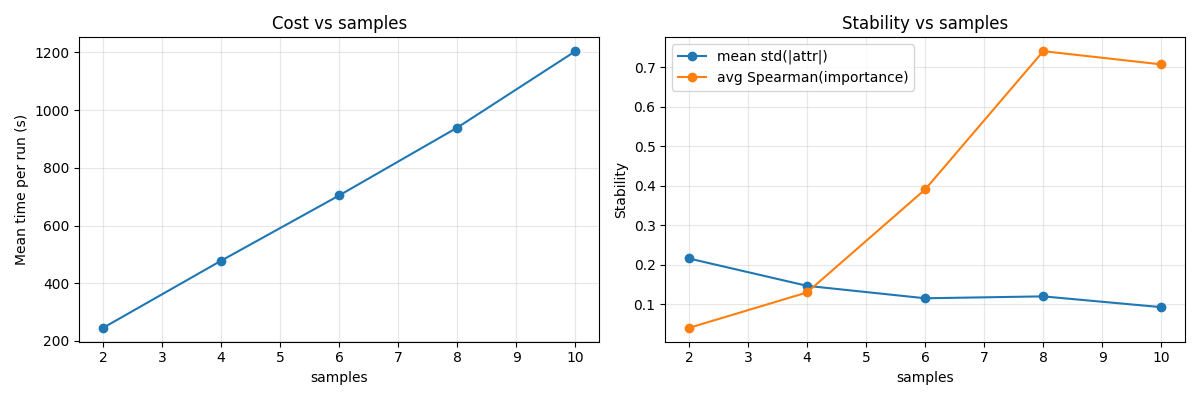
\includegraphics[width=0.95\linewidth]{ex3/ex3_cost_vs_quality.png}
    \caption{Koszt obliczeniowy i stabilność atrybucji w zależności od liczby próbek.}
    \label{fig:ex3_cost_vs_quality}
\end{figure}

\begin{figure}[H]
    \centering
    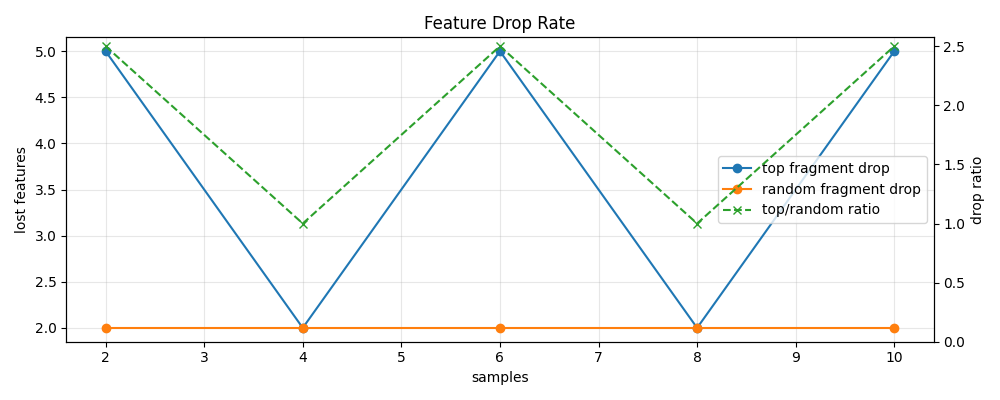
\includegraphics[width=0.95\linewidth]{ex3/ex3_feature_drop_rate.png}
    \caption{Feature Drop Rate dla fragmentu o najwyższej atrybucji i fragmentu losowego.}
    \label{fig:ex3_feature_drop_rate}
\end{figure}

Wyniki Feature Drop Rate potwierdzają użyteczność atrybucji, lecz nie widać wpływu liczby próbek: usunięcie fragmentu o najwyższej ważności zwykle powoduje większą utratę cech niż usunięcie fragmentu losowego. Dla 2 próbek top fragment powodował utratę 5 cech przy 2 cechach dla losowego baseline'u, a przy 6 i 10 próbkach zachowano tę samą przewagę (5 vs 2). Dla 4 i 8 próbek oba warianty dawały 2 utracone cechy, co sugeruje, że w tym przykładzie niektóre fragmenty są semantycznie zbliżone pod względem wpływu na architekturę.


\subsection{Eksperyment 4: Stabilność Atrybucji}

\paragraph{Cel:} Sprawdzenie, czy atrybucje są stabilne dla tego samego promptu uruchamianego wielokrotnie.

\paragraph{Metodyka:}
\begin{enumerate}
    \item Wybrany prompt uruchamiany jest wielokrotnie
    \item Dla każdego uruchomienia obliczane są atrybucje
    \item Analizowana jest wariancja atrybucji między uruchomieniami
    \item Sprawdzana jest zgodność rankingów fragmentów
\end{enumerate}

\paragraph{Metryki:}
\begin{itemize}
    \item Wariancja atrybucji: odchylenie standardowe wartości atrybucji. Obliczane osobno dla każdego feature'a, a następnie uśredniane.
    \item Zgodność rankingów: współczynnik Spearmana między rankingami fragmentów
    \item Stabilność: procent fragmentów, których ranking nie zmienia się między uruchomieniami
\end{itemize}

\paragraph{Wyniki:}

Eksperyment stabilności wykonano dla tego samego promptu wielokrotnie, korzystając ze skryptu. Dla każdej fragmentacji promptu obliczano atrybucje. Na tej podstawie wyznaczono wariancję oraz odchylenie standardowe wartości atrybucji dla każdego fragmentu.
\begin{itemize}
    \item Liczba uruchomień: \textbf{8}
    \item Średnia zgodność rankingów (średni współczynnik Spearmana, pairwise): \textbf{0.4556}
    \item Stabilność rankingów (procent fragmentów bez zmiany pozycji): \textbf{0.00\%}
\end{itemize}

% \begin{figure}[H]
%     \centering
%     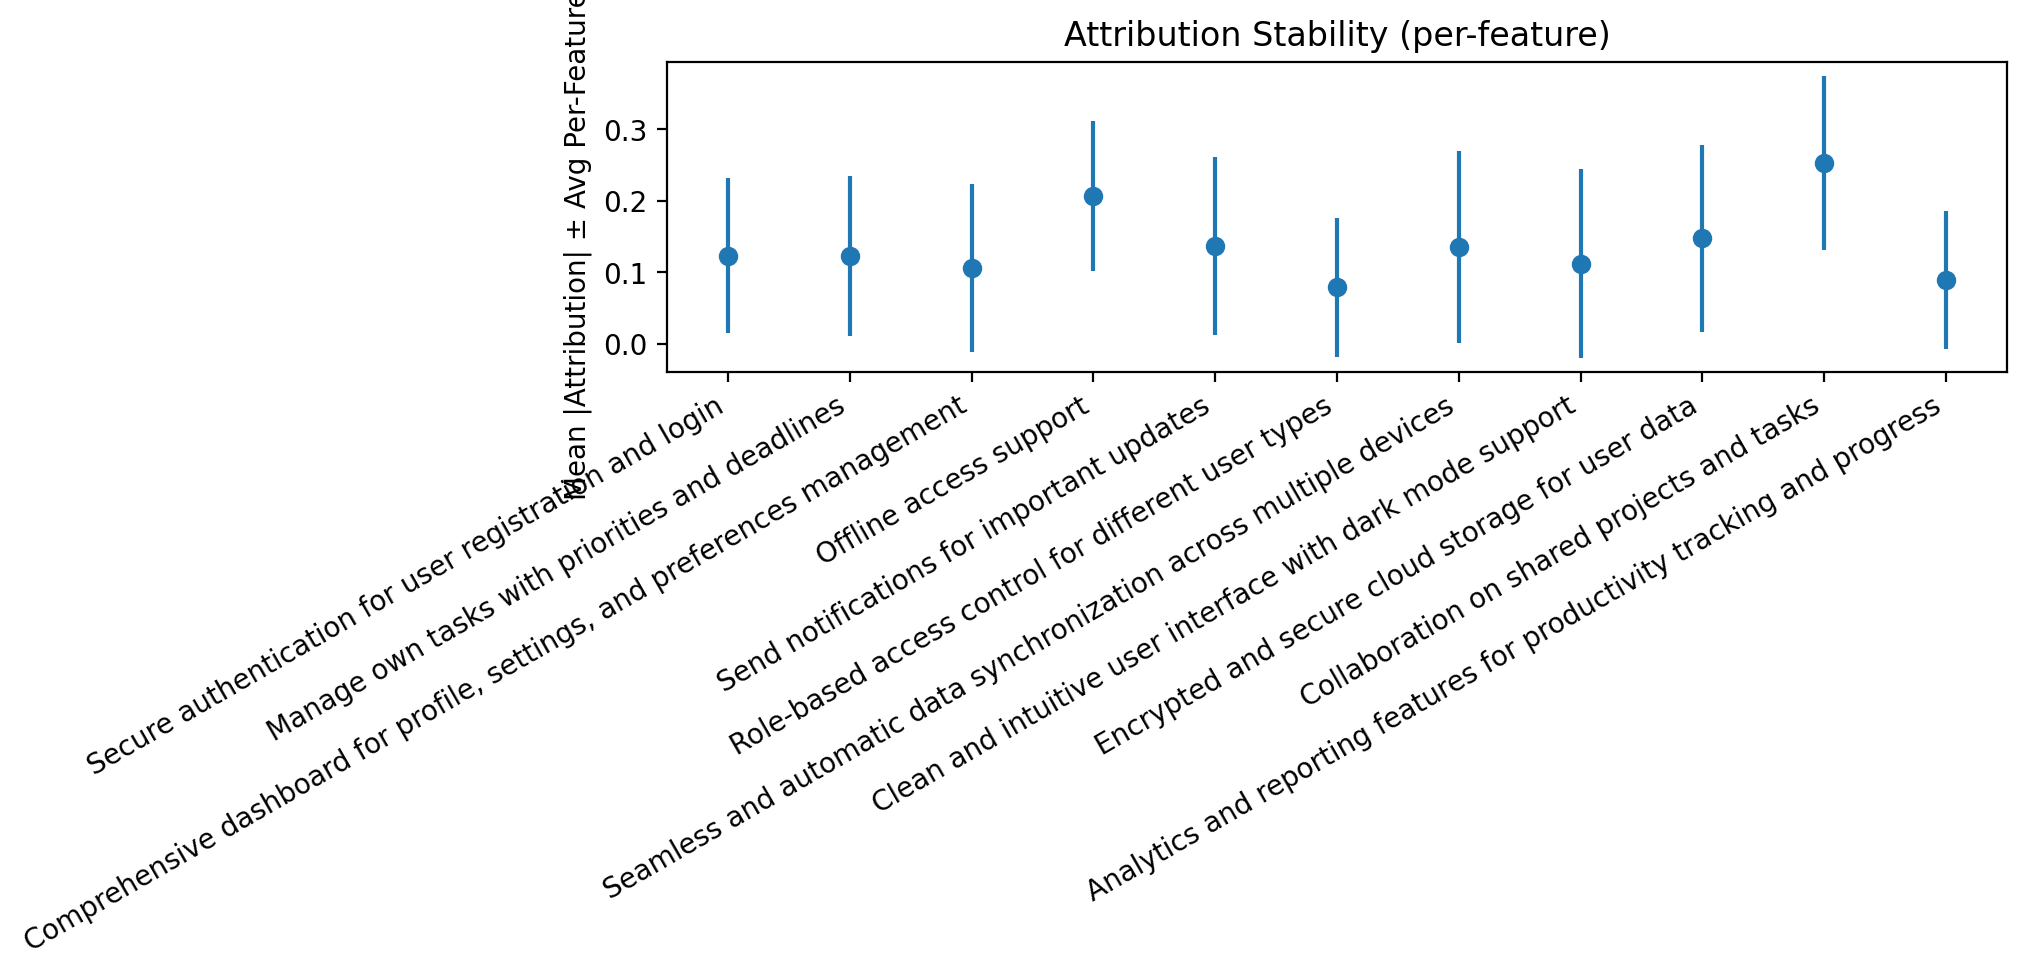
\includegraphics[width=1\linewidth]{ex4_stability.png}
%     \caption{Wykres stabilności atrybucji dla poszczególnych fragmentów promptu. Każdy punkt reprezentuje średnią atrybucję dla fragmentu (dla wszystkich feature'ów), a linie błędu pokazują odchylenie standardowe między uruchomieniami (obliczone osobno dla każdego feature'a, a potem uśrednione).}
%     \label{fig:ex4_stability}
% \end{figure}

Najbardziej niestabilne fragmenty według odchylenia standardowego wartości bezwzględnych atrybucji to:
\begin{itemize}
    \item \texttt{Seamless and automatic data synchronization across multiple devices} — std $\approx 0.135$
    \item \texttt{Clean and intuitive user interface with dark mode support} — std $\approx 0.132$
    \item \texttt{Encrypted and secure cloud storage for user data} — std $\approx 0.131$
    \item \texttt{Send notifications for important updates} - std $\approx 0.124$
    \item \texttt{Collaboration on shared projects and tasks} — std $\approx 0.121$
\end{itemize}

Średnie odchylenie standardowe dla wszystkich fragmentów wyniosło około $0.116$, co wskazuje na dość niską zmienność atrybucji między uruchomieniami.

\begin{figure}[H]
    \centering
    \includegraphics[width=1\linewidth]{ex4_least_stable.png}
    \caption{Wykres pokazujący stabilność atrybucji różnych feature'ów dla fragmentu "Seamless and automatic data synchronization across multiple devices", który był najbardziej niestabilny. Każdy punkt reprezentuje atrybucję dla danego feature'a, a linie błędu pokazują odchylenie standardowe między uruchomieniami.}
    \label{fig:ex4_least_stable}
\end{figure}

\paragraph{Interpretacja:}
\begin{itemize}
    \item Atrybucje nie są całkowicie deterministyczne, co jest zgodne z losowym charakterem sampling-based SHAP-inspired.
    \item Wartość stabilności rankingów równa $0.00\%$ oznacza, że każdy fragment zmienił pozycję przynajmniej raz pomiędzy uruchomieniami; nie oznacza to jednak całkowitego braku zgodności globalnej, co potwierdza średni Spearman równy $0.4556$.
    \item Najbardziej ogólne lub wieloznaczne fragmenty promptu mogą zmieniać swoje znaczenie pomiędzy uruchomieniami bardziej niż fragmenty jednoznacznie mapowane na feature'y.
    \item Stabilność wyników można poprawiać przez zwiększenie liczby próbek, ale kosztem czasu obliczeń.
\end{itemize}

\section{Wnioski}

\subsection{Główne Ustalenia}

Na podstawie przeprowadzonych eksperymentów można sformułować kilka spójnych wniosków.

Po pierwsze, atrybucja fragmentów promptu rzeczywiście pomaga wskazywać te elementy wejścia, które mają największy wpływ na wygenerowaną architekturę. Potwierdza to Eksperyment 1, w którym usunięcie najwyżej ocenionego fragmentu zwykle powodowało większą utratę cech niż usunięcie fragmentu losowego.

Po drugie, wyjaśnienia atrybucyjne są użyteczne w procesie refinementu promptu, ponieważ skracają drogę do poprawnego sformułowania wymagań i zmniejszają liczbę iteracji potrzebnych do osiągnięcia celu, choć nie zawsze skracają całkowity czas zadania.

Po trzecie, jakość wyjaśnień zależy od liczby próbek używanych w metodzie SHAP-inspired. Wyniki z Eksperymentu 3 pokazują wyraźny kompromis: większa liczba próbek poprawia stabilność i zgodność rankingów, ale znacząco zwiększa koszt obliczeniowy. Na tej podstawie zakres 6--8 próbek wydaje się najlepszym praktycznym kompromisem dla tego prototypu. Po czwarte, atrybucje nie są w pełni deterministyczne, co potwierdza Eksperyment 4. Oznacza to, że system nadaje się do wspomagania analizy i iteracyjnego dopracowywania promptów, ale nie powinien być traktowany jako źródło absolutnie stabilnego wyjaśnienia bez dalszego zwiększania liczby próbek lub zastosowania bardziej zaawansowanej metody estymacji.

Podsumowując, postawione pytania badawcze otrzymują częściowo pozytywną odpowiedź: atrybucja poprawia zrozumienie wpływu promptu na cechy aplikacji, wspiera refinement promptu i daje użyteczne sygnały diagnostyczne, ale wymaga ostrożnej interpretacji ze względu na koszt obliczeniowy i zmienność wyników.


\subsection{Przyszłe Prace}

\begin{itemize}
    \item Przeprowadzenie pełnych testów użytkowników
    \item Opracowanie interfejsu graficznego
    \item Eksploracja innych modeli językowych
    \item Analiza wpływu temperatury i różnych parametrów LLM
\end{itemize}


\begin{thebibliography}{99}

\bibitem{SHAP} Lundberg, S. M., \& Lee, S. I. (2017). A unified approach to interpreting model predictions. \textit{Advances in Neural Information Processing Systems}, 30.

\end{thebibliography}

\end{document}
